\documentclass[journal,10pt]{IEEEtran} 
\IEEEoverridecommandlockouts
\usepackage{lipsum}
%\documentclass[journal,onecolumn]{IEEEtran} 
%\documentclass[sigconf]{acmart}
%\usepackage[sorting=none,style=numeric]{biblatex}
%\usepackage{cite}
\usepackage{amsmath,amssymb,amsfonts}
\usepackage{algorithmic}
\usepackage{graphicx}
\usepackage{textcomp}
\usepackage{xcolor}
\def\BibTeX{{\rm B\kern-.05em{\sc i\kern-.025em b}\kern-.08em
    T\kern-.1667em\lower.7ex\hbox{E}\kern-.125emX}}

%-------------------------------- 0210
\usepackage[english]{babel}
\usepackage[square,numbers]{natbib}
\usepackage{longtable}
\usepackage{etoolbox}
\usepackage{amsmath,amssymb,amsfonts}
\usepackage{algorithmic}
\usepackage{graphicx}
\usepackage{textcomp}
\usepackage{xcolor}
\usepackage{natbib}
\usepackage[hyphenbreaks]{breakurl}
\usepackage[hyphens]{url}

\usepackage[utf8]{inputenc} % allow utf-8 input
\usepackage[T1]{fontenc}    % use 8-bit T1 fonts
\usepackage{hyperref}       % hyperlinks
\usepackage{url}            % simple URL typesetting
\usepackage{booktabs}       % professional-quality tables
\usepackage{amsfonts}       % blackboard math symbols
\usepackage{nicefrac}       % compact symbols for 1/2, etc.
\usepackage{microtype}      % microtypography

\usepackage{multirow}
\usepackage{makecell}
\usepackage{amsmath}        % new
\usepackage{amssymb}        % new
\usepackage{amsthm}
\usepackage{tikz}
\usepackage{pdfpages}
\usepackage{comment}
%\usepackage{cite}
%\usepackage{caption}
%\usepackage{subcaption}
\usepackage{flushend}
\usepackage[linesnumbered,ruled]{algorithm2e}
\usepackage[justification=centering]{caption}
%\usepackage[backend=biber,style=ieee, maxnames=10]{biblatex}

%For Verbatim fonts and sizes
\usepackage{fancyvrb}
\usepackage{datetime}
\newdate{date}{25}{01}{2023}
\date{\displaydate{date}}
%\date{\monthyeardate}

%\let\svmaketitle\maketitle
%\def\maketitle{\svmaketitle\thispagestyle{empty}}
%\markboth{Stanford CS372 Lecture Notes, 2020-22}%
%{Shell \MakeLowercase{\textit{et al.}}: Edward Y. Chang}

\newenvironment{noindlist}
 {\begin{list}{\labelitemi}{\leftmargin=0.3em \itemindent=0.6em}}
 {\end{list}}

 \newenvironment{noindenumerate}
  {\begin{list}{\arabic{enumi}.}
    {\usecounter{enumi}
     \setlength{\labelwidth}{0.6cm}
     \setlength{\leftmargin}{0.33cm}
     \setlength{\labelsep}{0.1cm}
     \setlength{\itemindent}{0cm}
     }
  }
  {\end{list}}
%\pagestyle{empty}
\begin{document}
\pagenumbering{gobble} 
\pagestyle{empty}
\title{Prompting Large Language Models \\ With the Socratic Method}

\author{Edward Y. Chang \\ Computer Science, Stanford University \\ echang@cs.stanford.edu%
% \thanks{}%
}

%\markboth{IEEE CWCC}{}
%\@anonymizetrue 

\maketitle


%\IEEEoverridecommandlockouts
%\IEEEpubid{\makebox[\columnwidth]{979-8-3503-3286-5/23/\$31.00 \copyright 2023 IEEE %\hfill} \hspace{\columnsep}\makebox[\columnwidth]{ }}

\pagestyle{empty}
\begin{abstract}
This paper presents a systematic approach to using the Socratic method in developing prompt templates that effectively interact with large language models, including GPT-3. Various methods are examined, and those that yield precise answers and justifications while fostering creativity and imagination to enhance creative writing are identified. Techniques such as {\em definition}, {\em elenchus}, {\em dialectic}, {\em maieutics}, {\em generalization}, and {\em counterfactual reasoning} are discussed for their application in engineering prompt templates and their connections to inductive, deductive, and abductive reasoning. Through examples, the effectiveness of these dialogue and reasoning methods is demonstrated. An interesting observation is made that when the task's goal and user intent are conveyed to GPT-3 via ChatGPT before the start of a dialogue, the large language model seems to connect to the external context expressed in the intent and perform more effectively.
\end{abstract}

\begin{IEEEkeywords}
large language model, natural language processing, prompting, the Socratic method.
\end{IEEEkeywords}

% Importance and appeal of children's drawings
Children's depictions of the human figure are highly expressive and varied.
As one of the very first subjects children attempt to draw, the representation begins as an almost unintelligible cloud of scribbles. 
As the child grows, their representation of the human figure becomes more developed and is extended to graphically represent many different types of characters: people, animals, and even personified objects (see Figure 1).

Who among us has not wished, either as a child or as an adult, to see such figures come to life and move around on the page?
Sadly, while it is relatively fast to produce a single drawing, creating the sequence of images necessary for animation is a much more tedious endeavor, requiring discipline, skill, patience, and sometimes complicated software.
As a result, most of these figures remain static upon the page.

% We built a system to animate them.
Inspired by the importance and appeal of the drawn human figure, we design and build a system to automatically animate it given an in-the-wild photograph of a child's drawing. 
Our system is fast, intuitive, and robust to much of the variation present in these types of drawings, making it well-suited to allow our target audience--children--to see their own characters coming to life.
The system is comprised of four stages: figure detection, segmentation masking, pose estimation/rigging, and animation. 
We describe each stage and identify common causes of failure in each. 
For object detection and pose estimation, we make use of existing computer vision models designed to detect human figures and joints in photographs; we fine-tune these models for use with children's drawings.
For segmentation, we present a straightforward, image processing-based method that, for animation purposes, is more useful and accurate than segmentation masks obtained from a fine-tuned object detection model.
During the animation step, we take advantage of the \textit{twisted perspective} commonly seen in children’s drawings to retarget motion capture data onto the character in a novel and appealing way.

% We use existing machine learning models. However, given the wide domain gap it's not clear how much fine-tuning data was needed. So we ran some experiments to find out and report it.
While our system leverages existing models and techniques, most are not directly applicable to the task due to the many differences between photographic images and simple pen and paper representations. 
To this end, we couple the presentation of our system with a set of experiments exploring the relationship between fine-tuning training set size and success rates.
We also include a perceptual study validating viewer preference for incorporating \textit{twisted perspective} into the motion retargeting step.

We validate the desirability and appeal of our system by building and publicly releasing a version of it as the \AD Demo \,\cite{animateddrawings}.
Launched in December 2021, this demo has been used by millions of people around the world to animate their children's drawings.
Inspired by this reception, our second contribution is The Amateur Drawings Dataset: \hjs{180,000 drawings and user-accepted annotations collected, with consent, through the demo. See Section \ref{sec:UI} for a description of how the annotations were generated.}
We believe this dataset will be a resource to researchers from various fields seeking to better understand the space of amateur drawings, evaluate new algorithms in this domain, or develop new drawing-based tools in general.

To summarize, our contributions are as follows:
\begin{enumerate}
    \item 
    We explore the problem of automatic sketch-to-animation for children's drawings of human figures and present a framework that achieves this effect. We also present a set of experiments determining the amount of training data necessary to achieve high levels of success and a perceptual study validating the usefulness of our motion retargeting technique.
    \item To encourage additional research in the domain of amateur drawings, we present a first-of-its-kind dataset of 180,000 user-submitted amateur drawings, along with user-accepted bounding box, segmentation mask, and joint location annotations.
\end{enumerate}

Upon acceptance of this paper, we plan to publicly release the Amateur Drawings Dataset, project code, and fine-tuned model weights.

\section{The Socratic method}
\label{sec:socratic}

The Socratic method is a questioning technique used in teaching and philosophy to encourage critical thinking and self-discovery \cite{SocraticMethidWiki}. The method involves asking a series of questions to explore complex ideas and help individuals arrive at their own understanding of a concept. It is based on the belief that knowledge cannot be simply imparted, but must be discovered through a process of questioning and dialogue.


Some of the Socratic method's key principles and guidelines to conduct critical thinking include:
\begin{noindlist}
\item Posing open-ended questions: The teacher or facilitator starts with a question to stimulate thinking and draw out ideas.
\item Clarifying key terms: The teacher helps the students clarify and define relevant terms and concepts to ensure everyone is on the same page.
\item Providing examples and evidence: The teacher or facilitator encourages the students to provide examples and evidence as reasons to support their claims.
\item Challenging reason-to-conclusion argument: The teacher or facilitator challenges the students' arguments and encourages them to question their own beliefs and to consider alternative perspectives.
\item Summarizing and drawing conclusions: The teacher helps the students summarize and draw conclusions from the discussion.
\item Reflecting on the process: The teacher and students reflect on the effectiveness of the method and what they learned through the dialogue.
\end{noindlist}

These principles of the Socratic method are realized through various methods and strategies. (Note the term ``method'' are used at the abstract level referring to the Socratic teaching
through questioning method, and his specific questioning techniques.) Some well-known examples of the Socratic method in action include Plato's ``Dialogues'' and ``Republic'' \cite{PaltoRepublicURL}, where Socrates uses questioning to  explore complex ideas and stimulate critical thinking in his interlocutors.

%\noindent
%\setlength{\leftskip}{-\parindent}
\begin{noindenumerate}
\item Definition: Socrates is known for his use of definition to clarify and explain the meaning of key terms and concepts.
\item Generalization: This method draws general principles from patterns that underlie observations and theories.
Generalization is used to form more certain and comprehensive conclusions.

\item Induction: Similar to generalization, but induction is based only on empirical evidence. Inductive reasoning provides hypotheses with high uncertainty.

\item Elenchus: This method involves cross-examination, where a series of questions is used to test the consistency and coherence of hypotheses and beliefs. Elenchus aims to 
test the validity of someone's arguments and to help them refine their thinking and eventually come up with well-supported hypotheses.

\item Hypothesis Elimination: This method involves eliminating false hypotheses and beliefs by testing them against counterexamples and logical reasoning.  Different from method elenchus, hypothesis elimination tests a hypothesis against evidence and logic to determine if it is true or false. 

\item Maieutics: This method involves helping individuals bring out the knowledge and understanding they already possess.
Maieutics is conducted by asking questions that encourage the person to reflect on their own experience, knowledge, beliefs and to explore alternative perspectives. Maieutics fosters  self-discovery, creative writing, and innovation.

\item Dialectic: This method involves exploring opposing viewpoints through dialogue or debate to arrive at a deeper understanding of a subject.

\item Recollection: This method involves the belief that knowledge is innate, and that people can remember what they already know through a process of questioning.

\item Irony: This method involves exposing ignorance and pretensions through irony, and pointing out the gap between claims and true understanding.

\item Analogy: This method involves comparing and contrasting different concepts through analogies, in order to help individuals understand complex ideas.
\end{noindenumerate}

%\subsection{Choices of Methods for Prompt Engineering}

At first glance, some reasoning methods may seem similar. For example, both induction and generalization use inductive reasoning, while both elenchus and hypothesis elimination use deductive reasoning. Similarly, methods like definition and dialectic use both inductive and deductive reasoning to explore opposing viewpoints through dialogue or debate. However, it is important to note that these methods have distinct differences, which will be discussed later in this paper.

In the context of critical thinking, methods like definition, elenchus, dialectic, hypothesis elimination, and generalization play active roles. On the other hand, during the brainstorming stage or in the context of creative thinking, methods like maieutics, induction, and counterfactual thinking are more relevant.

Analogy, irony, and recollection, are less relevant to our goal, so we do not consider them. Irony and analogy may not be necessary when working with language models, as these models may not understand figurative language. Recollection is limited by the memory of ChatGPT and GPT-3, which is a context window of $4k$ and $8k$, respectively. The prompter must use this limited space as context to allow the language model to recall information.


\begin{comment}
To improve input specificity, we suggest using the dialectic method with definition. The method of maieutics, combined with generalization and induction strategies, can be used to adapt a prompt template to the strengths of an LLM. The hypothesis elimination method can be used by all methods to remove information from low-reliability sources. Furthermore, we propose the addition of counterfactual reasoning \cite{NormTheory1986,FuncTheoryCounterfactual2008} to the list of methods. Counterfactual reasoning involves considering alternate outcomes of events, and the Socratic method can be used to guide discussions on this topic by encouraging critical thinking and self-reflection.
\end{comment}

\subsection{Illustrative Critical Reading Example}

To illustrate how these methods can practically be applied, let's use the example of critical reading. Critical reading is a crucial component of critical thinking, which involves evaluating the quality and credibility of written materials, from research papers to blog posts \cite{lai-etal-2017-race,PaulBinkerCT1990}. It requires a systematic and analytical approach, asking relevant questions, and using effective prompts to gain deeper understanding of the text \cite{Elder2010}.


\begin{table}[ht!]
%\vspace{-.1in}
\begin{center}
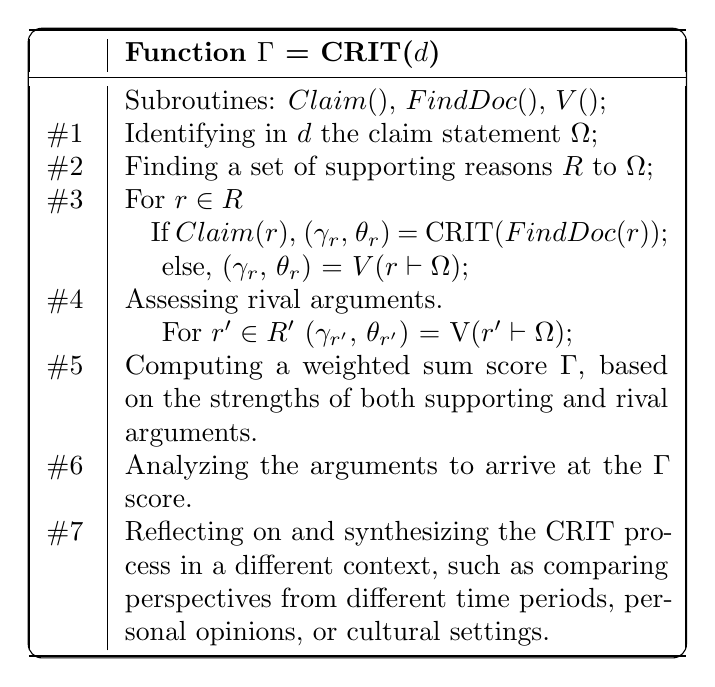
\begin{tikzpicture}
\node (table) [inner sep=0pt] {
\begin{tabular}{|p{0.56cm}|p{6.9cm}|}
\toprule
\textbf{} & \textbf{Function $\Gamma$ = CRIT($d$)} \\
\midrule
%& Function $\Gamma$ = CRIT($d$); \\
& Subroutines: $Claim$(), $FindDoc$(), $V$(); \\
\#1 & Identifying in $d$ the claim statement $\Omega$; \\
\#2 & Finding a set of supporting reasons $R$ to $\Omega$; \\
\#3 & For $r \in R$ \\
& ~~~~{If} $Claim$($r$), ($\gamma_r$, $\theta_r$) = CRIT($FindDoc$($r$)); \\
& ~~~~{else}, ($\gamma_r$, $\theta_r$) = $V$($r \vdash \Omega$); \\
\#4 & Assessing rival arguments. \\
& ~~~~For $r' \in R'$ ($\gamma_{r'}$, $\theta_{r'}$) = V($r' \vdash \Omega$); \\
\#5 & Computing a weighted sum score $\Gamma$, based on the strengths of both supporting and rival arguments. \\
\#6 & Analyzing the arguments to arrive at the $\Gamma$ score. \\
\#7 & Reflecting on and synthesizing the CRIT process in a different context, such as comparing perspectives from different time periods, personal opinions, or cultural settings. \\
\bottomrule
\end{tabular}
};
\draw [rounded corners=.5em] (table.north west) rectangle (table.south east);
\end{tikzpicture}
\end{center}
\caption{CRIT Pseudo-code. Input $d$ document, output $\Gamma$ validation score, V() validation routine, $R$ reason set, $R'$ rival reason set, ($\gamma_{r}$, $\theta_{r}$) validity and credibility scores of $r \vdash \Omega$.}
\label{tab:CRIT}
%\vspace{-.2in}
\end{table}


To aid in critical reading, we introduce a template called CRIT, which stands for Critical Reading Inquisitive Template. Given a document $d$, CRIT evaluates it and produces a validation score $\Gamma$. Let $\Omega$ denote the conclusion or claim of $d$, and let $R$ be the set of reasons supporting the claim. We define ($\gamma_r, \theta_r$) = V($r \vdash \Omega$) as the causal validation function, where $\gamma_r$ denotes the validation score $\theta_r$ the source credibility score and for each reason-to-conclusion entailment $r \vdash \Omega$. Table~\ref{tab:CRIT} presents the pseudo-code of $\Gamma$ = CRIT($d$), which generates the final validation score for document $d$ with justifications.

In the following sections, we will discuss five methods: 1) definition, 2) elenchus, 3) dialectic, 4) maieutics, and 5) counterfactual thinking.


\subsection{Method of Definition}

As shown in the pseudocode in Table~\ref{tab:CRIT}, 
the CRIT algorithm starts in
its step $\#1$, asking GPT-3 to identify the conclusion of a document. To avoid any misunderstandings, the prompt includes a clear instruction and definition. (In the square brackets, {\em in} denotes a input slot to an LLM and {\em out} the output slot.)

\begin{table}[ht!]
\small
\begin{tabular}{p{0.6cm}|p{7.2cm}}
p1.1 & ``What is the conclusion in document [in: $d$] 
  [out: $\Omega$]? \\ 
& The conclusion statement may 
  be written in the last paragraph, near 
  keywords "in conclusion," "in summary," or "therefore."'' \\
\end{tabular}
\end{table}

We can use
the {\em definition} method to 
improve the understanding of the document. 
One approach is paraphrasing the prompt 
into multiple prompts and grouping them into an ensemble, similar to forming a thesis committee. (Section~\ref{sec:template} presents
prompt ensemble in details.)
Different members can phrase the same question in different ways or ask it from a different perspective.  For example:

\begin{table}[h!]
\small
\begin{tabular}{p{0.6cm}|p{7.2cm}}
p1.2 &  ``What is the issue addressed by [in: $d$] 
  [out: $\Omega$]?'' \\
p1.3 & ``What is the most important outcome presented in text [in: $d$]? [out: $\Omega$]''
\end{tabular}
\end{table}

Step $\#2$ in Table~\ref{tab:CRIT} prompts 
GPT-3 to find a set of
supporting reasons.  Similarly, the prompt can
be ``evidences'', ``opinions'', in addition to
``reasons'' to query for the document's 
support to its conclusion.

\begin{table}[ht!]
\small
\begin{tabular}{p{0.6cm}|p{7.2cm}}
p2 & ``What are the supporting reasons [out: $R$] of conclusion \\
& [in: $\Omega$] of [in: $d$]?'' 
\end{tabular}
\end{table}

\begin{comment}
Note that prompts can be submitted all together or
one-by-one to GPT-3. Our empirical study 
on reading comprehension
samples~\cite{501Q2004} shows that issuing prompts one-by-one
generates output with finer details.  This is because
GPT-3 has a chance to examine a document multiple times
for slightly different purposes.
For teaching K-12 students critical reading, 
the one-by-one prompting is
better because it allows students to interact with
CRIT step-by-step.  
\end{comment}

\subsection{Method of Elenchus}

The method of elenchus is rooted in the Greek word ``elenchein,'' which translates to examine. This method involves cross-examining the results generated by GPT-3 to evaluate the consistency and coherence of the arguments. The goal is to arrive at a deeper understanding of the validity of the reasons and conclusion, and to identify any potential weaknesses or flaws in the arguments.

Step $\#3$ of the CRIT algorithm (in Table~\ref{tab:CRIT}) prompts GPT-3 to assess the validity of each reason $r \in R$ as justification for the conclusion $\Omega$ through the function V($r \vdash \Omega$). To validate the reason-to-conclusion argument, CRIT must evaluate the presented reason and its causal relationship with the conclusion and conduct cross examination, which is precisely the task of the method of elenchus.

CRIT issues four prompts to evaluate the logic validity and source credibility of the $r \vdash \Omega$ entailment. Prompt $\#3.2$ elicits supporting evidence for reason $r \in R$. This evidence can be a theory, an opinion, statistics, or a claim from other sources. If the reasoning is a claim, then the sources that the claim is based on are recursively examined. The strength of the argument and its source credibility are rated on a scale of $1$ to $10$, with $10$ being the strongest.


\begin{table}[h!]
\small
\begin{tabular}{p{0.6cm}|p{7.2cm}}
p3.1 & ``What is the evidence for reason [in: $r$] to support
conclusion [in: $\Omega$] in document [in: $d$]? [out: evidence]'' \\ 
p3.2 & ``What is the type of evidence? A) a theory, B) an opinion, C) statistics, or {\color{red}D}) a claim from other sources?'' \\
p3.3 & ``If the evidence of reason [in: $r$] is {\color{red}D}),
  call CRIT recursively to extract supporting reasons [out: $R'$].'' \\
p3.4 & ``How strongly does reason [in: $r$] support
  [in: $\Omega$] in document [in: $d$]? Rate argument validity [out: $\gamma_v$] and source credibility [out: $\gamma_c$] between $1$ and $10$ (strongest).''
\end{tabular}
\end{table}


It may be beneficial to also incorporate the counter-argument method in order to gain a more comprehensive and balanced evaluation of the argument. This can result in a deeper understanding of the topic being discussed. We will be discussing this further in the next section.

\begin{comment}
\begin{table}[h!]
\small
\begin{tabular}{p{0.6cm}|p{7.2cm}}
\end{tabular}
\end{table}
\end{comment}

\subsection{Method of Dialectic}

The easiest way to mislead without lying outright is to leave out critical counterarguments from the reader.
CRIT relies on GPT-3 to generate and
evaluate counter arguments, similar to
how it prompts GPT-3 to extract and 
evaluate reasons. 

CRIT in its step $\#4$ asks GPT-3 to provide missing
rival reasons, and then pair rival reasons
with the conclusion to conduct validation.
There are two strategies to 
bring counter arguments to the surface.
The first strategy attacks the weakest 
arguments with the lowest scores and asking
GPT-3 to attack those entailment's.

\begin{table}[h!]
\small
\begin{tabular}{p{0.6cm}|p{7.2cm}}
p4 & ``Are there counter counterargument against [in: $r \vdash \Omega$] in [in: $d$]? If so, provide counter reasons [output $R'$].''
\end{tabular}
\end{table}

For finding omitted information, CRIT can
query GPT-3 without quoting any $r \in R$,
and follow the same process. At the end,
CRIT can append to the $\gamma$ score with
a $-\gamma$ score, and provide 
an alert to the reader with a 
a summary of the counter argument. 

Finally, in step $\#5$, CRIT computes an aggregated 
score by performing a weighted sum on
the validation multiplied by credibility score,
of both arguments and counter arguments, and then
output the final assessment score $\Gamma$.

\begin{table}[h!]
\small
\begin{tabular}{p{0.6cm}|p{7.2cm}}
p5 & ``Final score [out: $\Gamma$]. $\Gamma = 
\sum_{r \in R \cup R'} \gamma_r \times \theta_r / |R \cup R'|$.
\end{tabular}
\end{table}
%\noindent
%\subsubsection*{Remarks on Critical Reading vs. Thinking} 
%\hfill \break



\subsection{Method of Maieutics}
\label{sec:Maieutics}

The maieutic method derives from the Greek word ``maieutikos,'' meaning midwife. It is founded on the belief that a teacher's role is to facilitate students in bringing forth their own understanding of a subject, rather than simply conveying knowledge. Unlike the elenctic method, which aims to detect and eliminate false hypotheses, maieutics centers on helping students reveal their own understanding of a subject. In this dialogical method, the teacher asks questions that are intended to guide the student in discovering their own comprehension, rather than providing them with information or answers.

Moving on to GRIT, after the text has been scored in step $\#5$, it is valuable for readers or students to summarize and analyze the justifications produced by GPT-3 to enhance their analytical and writing skills. CRIT can prompt GPT-3 for a report, and then readers and students can compare their notes.

\begin{table}[h!]
\small
\begin{tabular}{p{0.6cm}|p{7.2cm}}
p6 & ``For every $r \in R \cup R'$ justify the validity score $\gamma_r$ and source credibility score $\theta_r$ for
each entailment $r \vdash \Omega$.''
\end{tabular}
\end{table}


\subsection{Counterfactual Reasoning}
\label{sec:cf}

Counterfactual reasoning~\cite{Cross-Examination2021,WinArgument2006} can be seen as a natural extension of the Socratic method, as both involve questioning assumptions and exploring alternative perspectives. 
Counterfactual thinking involves imagining alternative scenarios to what actually happened, often using phrases like ``what if'' or ``if only.''
By incorporating counterfactual reasoning into prompt engineering, one can facilitate exploration of alternative possibilities and promote more nuanced and complex understanding of a given topic.

The final step of GRIT involves using the counterfactual method to encourage students to reconsider the arguments and counterarguments presented in the text based on new contextual information. CRIT can prompt students with questions such as ``what if the debate in the text took place now instead of in the 1950s?'' or ``what if the main event in the text occurred in Asia instead of in Europe?'' Students can express their own opinions and findings based on further reading and statistics, and challenge the conclusions drawn in the text. Table~\ref{tab:CRIT} lists three contexts for consideration: when, who, and where.


\subsection{Remarks on the Socratic Method and CRIT}

As we have shown that for critical reading,
GRIT uses three methods, definition, elenchus, and dialectic.  
For critical thinking, CRIT uses methods maieutics and counterfactual reasoning. For more explorative 
thinking, 
methods such as induction can be used for informal brainstorming, hypothesis elimination for removing weak propositions, and generalization for deriving principles from examples.

Please note that prompts can be submitted to GPT-3 either all together or one-by-one. Our empirical study on reading comprehension samples~\cite{501Q2004} demonstrates that issuing prompts one-by-one results in outputs with finer details. This is because GPT-3 has the opportunity to analyze a document multiple times for slightly different purposes. For teaching critical reading to K-12 students, one-by-one prompting is preferred as it allows students to engage with CRIT step-by-step.

\begin{comment}
\begin{small}
\begin{verbatim}
\end{verbatim}
\end{small}
\end{comment}


\section{Prompt Template Engineering}
\label{sec:template}

Prompt template engineering involves creating templates to provide input, or ``prompts,'' to a language model to guide its output generation. In this section, we discuss prompt template engineering methods for basic building blocks, and then integrate the methods of definition, elenchus, dialectic, maieutics, and counterfactual reasoning to compose more complex templates. We present experimental results using different types of documents to demonstrate how the Socratic method can improve the accuracy and conciseness of the output through arguments and verification, as well as facilitate guided generalization and creativity.

\subsection{Basic, One Shot Template}

Let's begin by discussing a simple one-shot prompt template. In the work of \cite{SocraticModels-Google2022}, a simple formulation function is used to generate the prompt $x'$, which is obtained by applying the function $f_{prompt}(x)$ to the input $x$.

For machine translation, the prompt template can take the form of ``Translate from [Lan$_{from}$]: [X] to [Lan$_{to}$]: [Y],'' where Lan$_{from}$ can be either detected by the prompt template or identified by the LLM. The input $x$ provides the information to fill in the slots [X] and [Lan$_{to}$]. For example, if the input is ``translate good morning to French,'' the prompt template $x'$ would be ``Translate from English: 'good morning' to French: [Y].'' The empty slot [Y] is then filled with the LLM's output, such as ``bonjour.'' In cases where the LLM produces multiple responses, it can also provide a score for each, which the prompt template can use to select the highest-scoring response or to request a summary from the LLM.


There are three main design considerations when engineering a basic prompt. 
\begin{noindenumerate}
\item {Input style}. It is important to consider how to phrase the template so that it can handle different styles of user input for the same task. For example, a user may ask for a translation task to be performed by saying ``Translate $x$ to French,'' or ``What is the French translation of $x$?''
\item {LLM capability}. As discussed in \cite{PromptSurvey2023}, it is important to take into account the patterns and capabilities of the partner language model (LLM) when designing the template, such as whether the LLM is left-to-right \cite{OpenAI-GPT3-2020} or masked \cite{Devlin2019BERTPO}.
\item {Cost}. Certain tasks, such as language detection and summarization, can be performed by the template itself or by the LLM. The decision of whether to perform a task within the prompt template or to use the LLM should be based on factors such as cost.
\end{noindenumerate}

To address the first two technical challenges, one can start by hand-engineering a few seed templates and then paraphrasing them into an ensemble \cite{Haviv2021BERTeseLT}. We believe that the basic, one-shot formulation can always be replaced by an ensemble formulation \cite{Peng2022ModelEI, Schick2020ExploitingCF} and then learn the weights of its members for each query instance to produce the final output. Additionally, by examining which basic prompts have high weights, an ensemble with various paraphrased prompts can identify what an LLM knows, which can help infer its strengths without having to conduct capability
mining on the LLMs.

%\noindent
%{\color{blue} Note} Experiment idea: evaluate LLMs using ensembles.

\subsection{Prompt Clarification with Method Definition}
\label{sec:template-definition}

There are computer algorithms that can already be used to recursively clarify a question, its definitions, and sub-terms' definitions. In fact, the natural language processing (NLP) community has developed a large 
number of useful methods and algorithms over the years \cite{NLP-Text-JM3}. 
One can use NLP techniques, such as dependency parsing and named-entity recognition (NER) \cite{NLPScratch2011}, to analyze the structure and meaning of a question and identify key terms and concepts. For example, 
NER can be used to extract entities in user input, such as names, locations, and organizations, and co-reference resolution can be used to understand the referred entity of a pronoun. 
Before submitting a template to an LLM, the application (e.g., a chatbot) 
that uses the template should check if all input slots are filled, 
and perform a sanity check. In the translation example, if the [Lan$_{to}$] was not provided or the specified language is not supported by the LLM, then the application should inquire the user for clarification.

Regarding mapping a natural language input to a prompt template, existing techniques of knowledge representation and reasoning can be very helpful. More specifically, ontology alignment and semantic parsing \cite{Campagna2020AFS,zhou-etal-2021-structure} can help map an NL input to a structured representation of knowledge and infer implicit concepts and relationships. These algorithms can be used to generate more precise and accurate prompts for LLMs, and to improve the effectiveness of the Socratic method in dialogue formulation \cite{DialoguewithAttention2023}. Some available tools include NLTK (Natural Language Toolkit) and spaCy for NLP\footnote{spaCy (https://spacy.io/)}, and TensorFlow for ML\footnote{TensorFlow (https://www.tensorflow.org/)}.

%\noindent
%{\color{blue} Note} Experiment idea: compare w/ and w/o.

\subsection{Prompt Verification with Method Elenchus}

The main purposes of conducting cross examination in a template are to validate the credibility of the information sources and to identify inconsistencies in the process. Cross examination is typically conducted through a multi-turn dialogue \cite{DialoguewithAttention2023}. In the context of template engineering, the goal is to formulate a productive dialogue that can be used to assess the reliability of an LLM's output.  

There are several methods that can be used to assess and strengthen the reliability of an LLM's output. 1) The first approach is to paraphrase a question in order to obtain different answers and identify inconsistencies, if they exist, in multiple answers. 2) The second method is to ask for further evidence, such as querying top-k sources of information and asking the LLM to rate the credibility of each source. This can be used to compute the reliability of the output. 3) Additionally, template engineering can be used to query an LLM for opposing views of its output, including sources and credibility, and then evaluate if a different perspective is strong.

The implementation of the first two methods for cross examination, paraphrasing a question and asking for further evidence, is readily covered by the techniques enumerated in Section~\ref{sec:template-definition}. To implement the third method of asking for different perspectives, a simple approach is to find the sentiment of the original question and then rewrite the question with an opposite sentiment. For example, if the original question is phrased in a positive tone, the prompt template can reformulate the question with a negative tone to elicit a contrasting viewpoint.
A more elaborate method is to identify the people and sources in the LLM-generated responses and then re-post the questions to those who have a reputation for having different views. For example, if the original answer came from a democratic right-leaning source, the prompt template may post the same question to a source of a republican-left persuasion, and vice versa. This approach allows for a more comprehensive examination of the topic by considering multiple perspectives.

The template to examine the semantic relation between two sentences $S_1$ and $S_2$ can be 
written as ``<$S_1$>, [R], [$S_2$],'' where R
is one of the three most important 
types of semantic relations: paraphrase, entailment, and contradiction \cite{PTRSUN2021}. Two sentences that have the same meaning are called paraphrases of each other. Two sentences that
have different meanings can be called 
disagreement or contradiction. The template 
can be trained to identify the degree
of agreement (or disagreement) between two
sentences.  


Table \ref{tab:Elenchus} shows two examples of this. In the first example (shown on the top portion of the table), the prompter asks GPT-3 to confirm if James Watson and Francis Crick are the only contributors to the discovery of the DNA double helix structure. GPT-3 replies by mentioning two other contributors. The second example in the table asks GPT-3 to provide not only the answer to a question but also its information sources and rate the credibility of each source according to the prompter's specification. Although the reliability of GPT-3's ratings remains to be validated, this rating mechanism can serve as an alert when some sources are found to be unreliable.


\begin{table}[htbp!]
%\vspace{-.12in}
%\resizebox{\textwidth}{!}
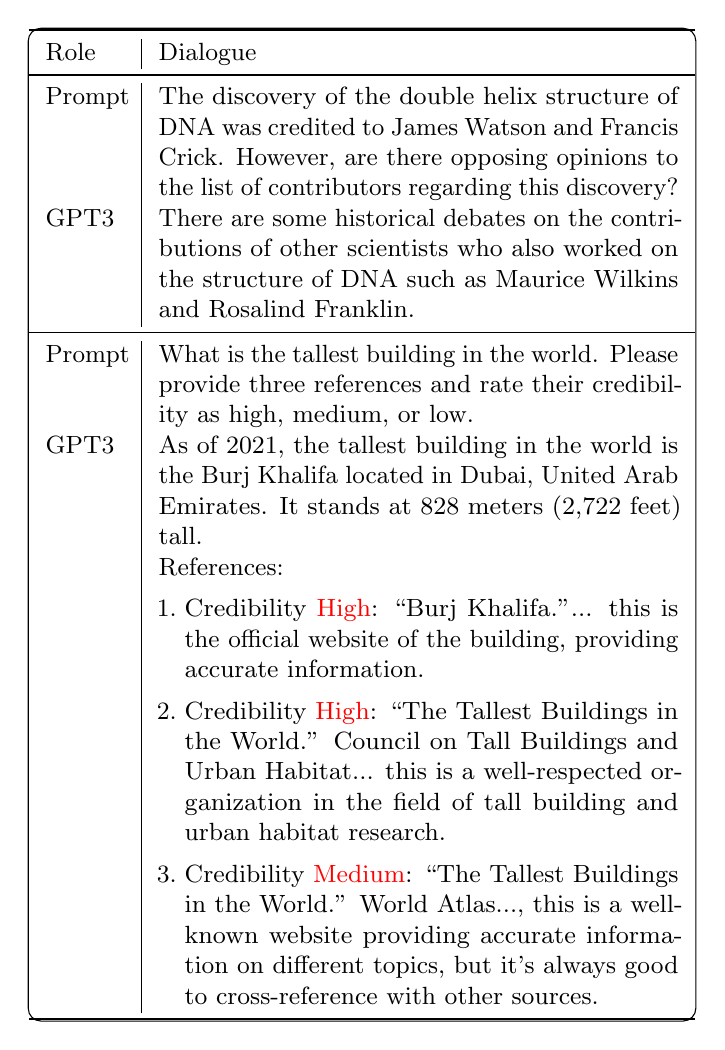
\begin{tikzpicture}
\begin{small}
\node (table) [inner sep=0.1pt] {
\begin{tabular}{p{1.0cm}|p{6.6cm}}
\toprule
Role & Dialogue \\
\midrule
Prompt & {The discovery of the double helix structure of DNA was credited to James Watson and Francis Crick. However, are there opposing opinions to the list of contributors regarding this discovery?}\\

GPT3 & {There are some historical debates on the contributions of other scientists who also worked on the structure of DNA such as Maurice Wilkins and Rosalind Franklin.} \\ 
\midrule 

Prompt & 
{What is the tallest building in the world.  Please provide three references and rate their credibility as high, medium, or low.} \\

GPT3 & {As of 2021, the tallest building in the world is the Burj Khalifa located in Dubai, United Arab Emirates. It stands at 828 meters (2,722 feet) tall.

References:
\begin{noindenumerate}
\item Credibility {\color{red}High}: ``Burj Khalifa.''... 
 this is the official website of the building, providing accurate information.
\item Credibility {\color{red}High}: ``The Tallest Buildings in the World.'' Council on Tall Buildings and Urban Habitat... this is a well-respected organization in the field of tall building and urban habitat research.
\item Credibility {\color{red}Medium}: ``The Tallest Buildings in the World.'' World Atlas..., 
this is a well-known website providing accurate information on different topics, but it's always good to cross-reference with other sources.
\end{noindenumerate}
} \\
\bottomrule
\end{tabular}
};
\draw [rounded corners=.5em] (table.north west) rectangle (table.south east);
\end{small}
\end{tikzpicture}
\caption{Examples of Method Elenchus.}
\label{tab:Elenchus}
\vspace{-.1in}
\end{table}


\subsection{Prompt Generalization with Method Maieutics}


\begin{table}[htbp]
%\resizebox{\textwidth}{!}
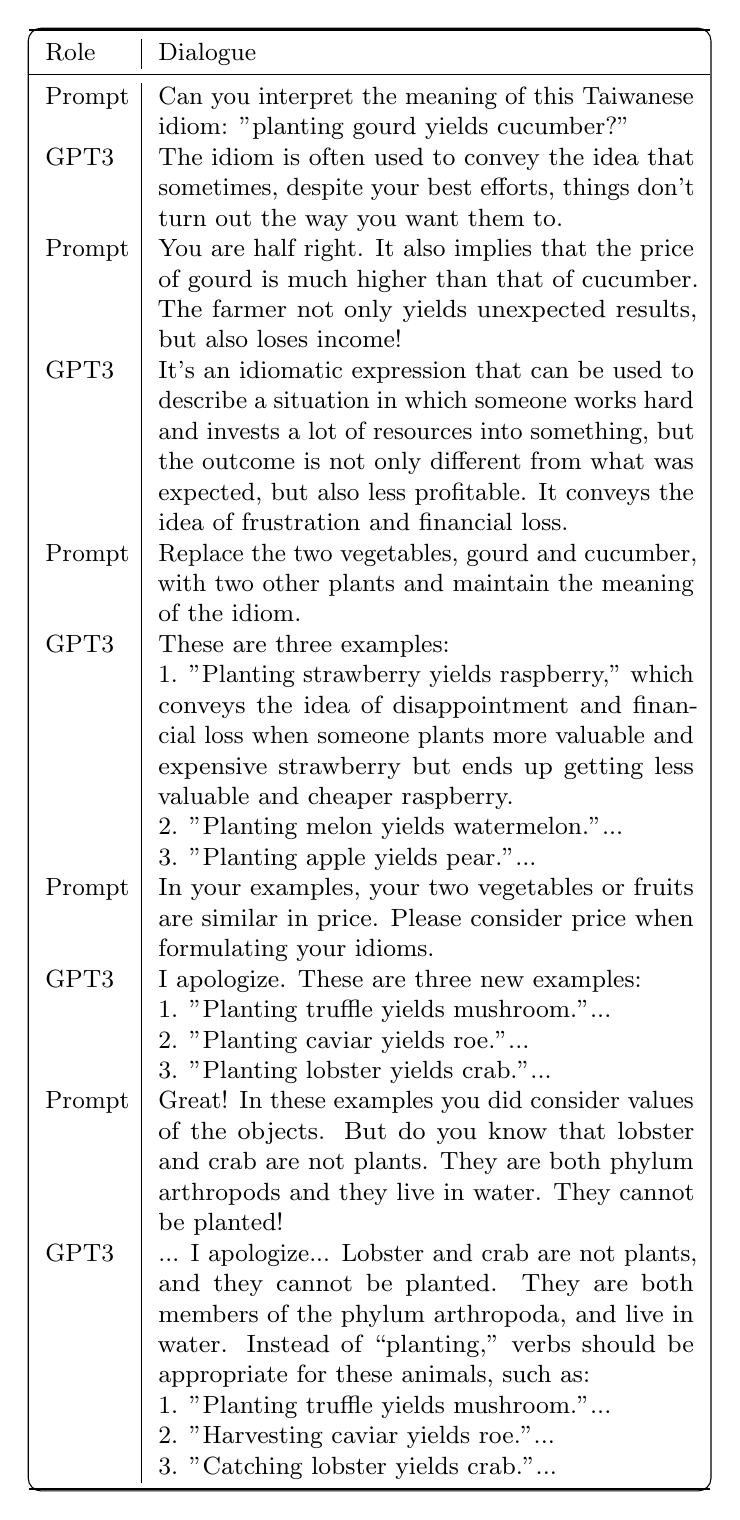
\begin{tikzpicture}
\begin{small}
\node (table) [inner sep=0pt] {
%\setlength\tabrowsep{1.5pt}
\begin{tabular}{p{1.0cm}|p{6.8cm}}
\toprule
Role & Dialogue \\
\midrule
Prompt & {Can you interpret the meaning of this Taiwanese idiom: "planting gourd yields cucumber?"}\\
GPT3 & {The idiom is often used to convey the idea that sometimes, despite your best efforts, things don't turn out the way you want them to.} \\
Prompt & {You are half right. It also implies that the price of gourd is much higher than that of cucumber. The farmer not only yields unexpected results, but also loses income! } \\

GPT3 & {It's an idiomatic expression that can be used to describe a situation in which someone works hard and invests a lot of resources into something, but the outcome is not only different from what was expected, but also less profitable. It conveys the idea of frustration and financial loss.} \\

Prompt & {Replace the two vegetables, gourd and cucumber, with two other plants and maintain the meaning of the idiom.} \\

GPT3 & {These are three examples:} \\
& 1. "Planting strawberry yields raspberry," which
conveys the idea of disappointment and financial loss when someone plants more valuable and expensive strawberry but ends up getting less valuable and cheaper raspberry. \\
& 2. "Planting melon yields watermelon."... \\
& 3. "Planting apple yields pear."... \\

Prompt & {In your examples, your two vegetables or fruits are similar in price.  Please consider price when
formulating your idioms.} \\

GPT3 & {I apologize. These are three new examples:} \\
& 1. "Planting truffle yields mushroom."... \\
& 2. "Planting caviar yields roe."... \\
& 3. "Planting lobster yields crab."... \\

Prompt & {Great! In these examples you did consider values of the objects. But do you know that lobster and crab are not plants. They are both phylum arthropods and they live in water. They cannot be planted! }  \\

GPT3 & {... I apologize... Lobster and crab are not plants, and they cannot be planted. They are both members of the phylum arthropoda, and live in water. Instead of ``planting,'' verbs should be appropriate for these animals, such as:} \\
& 1. "Planting truffle yields mushroom."... \\
& 2. "Harvesting caviar yields roe."... \\
& 3. "Catching lobster yields crab."... \\
\bottomrule
\end{tabular}
};
\draw [rounded corners=.5em] (table.north west) rectangle (table.south east);
\end{small}
\end{tikzpicture}
\caption{Example of Method Maieutics.}
\vspace{-.1in}
\label{tab:Maieutics}
\vspace{-.15in}
\end{table}


The example shown in Table~\ref{tab:Maieutics}, ``planting gourd yields cucumber,'' requires GPT-3 to first learn to select two produce objects, either vegetables or fruit, as input. The template is ``The farmer was so sad because he [verb] [X] but yields [Y], where price(X) >> price(Y).'' The first attempt may not strongly convey the condition price(X) >> price(Y), but with a few training iterations, GPT-3 started to ``recognize'' the price constraint and could also provide justifications when arguing for the price of tea being much higher than the price of spinach (not presented in the table).

Interestingly, after GPT-3 learned the price constraint, it started suggesting food items other than produce, such as caviar, roe, lobster, and crab. While the price constraint was observed, the verb ``plant'' is incorrect. Here, we suggest making the hard-coded verb ``plant'' an output slot: ``The farmer was so sad because he [verb] [X] but yields [Y], where price(X) >> price(Y).'' Amazingly, GPT-3 is able to fill in the slot with accurate verbs:

\begin{noindlist}
\item ``Harvesting (planting) truffle yields mushroom.''
\item ``Fishing (harvesting) for caviar yields roe.''
\item ``Trapping (catching) lobster yields crab.''
\end{noindlist}

This example demonstrates that GPT-3 can generate novel examples based on a template. When it suggests food items other than produce, it could be seen as an error as the boundary set by the verb ``plant'' is violated. However, this could also be seen as an innovative act by GPT-3, extending the constraint hinted by the verb. Impressively, the new examples still preserve the original intent of showing a producer's emotional distress.

How can this guided generalization be accurately and automatically performed to edit a template? Socrates' method of generalization starts with specific instances and then draws general statements from them. The procedure for generalization involves identifying common patterns or themes in a set of examples, and then formulating a general rule that captures these patterns. In the example presented in Table~\ref{tab:Maieutics}, we started by asking GPT-3 to meet the price(X) >> price(Y) constraint, with the condition that X and Y must both be produce grown in soil. However, upon analyzing GPT-3's outputs, we discovered that some instances of X and Y were not produce (e.g., lobster and caviar). This finding led to the realization that the hard-coded verb ``plant'' in the template was too restrictive. To address this issue, we applied generalization by allowing the [verb] slot to be open, making the template statement more general. In this case, the mistakes made by GPT-3 served as valuable training data, allowing us to generalize the original template and make the expression more vivid and dynamic.

\subsection{Prompt Exploration with Counterfactual Reasoning}

Imagination and creating novel plots are crucial for writers, as it allows for ``creative freedom'' and ``artistic license.'' Creativity is the ability to think differently and approach problems with fresh and imaginative ideas.

However, an imagination without a clear subject matter, scope, or a story line can lead to a lack of productivity. To captivate the audience, a writer must consider human experiences and emotions as constraints. Therefore, ``creative freedom'' should not be viewed as total freedom, but rather as the ability to condition future narratives in the context and to create plots that turn and twist in unexpected ways.

The technique of counterfactual \cite{Pearl2009} can be useful in guiding imagination. It involves considering alternative scenarios and outcomes. This can lead to the exploration of different possibilities and the generation of new and unique plot ideas. For example, a writer may ask ``what if'' questions to change the narrative of events, such as ``what if the main character had not fallen in love?'' or ``what if an accident occurred on the way to a highly-anticipated date?'' By considering these counterfactuals, a writer and an LLM can create more engaging and interesting stories. One can ask an LLM to generate several scenarios and then select the most suitable one for the writer to continue writing.

We have experimented with using the counterfactual technique to
rewrite chapters in Chinese classical novels, ``Outlaws of the Marsh'' and ``Dream of the Red Chamber.'' We have also asked GPT-3 to rewrite Genesis chapter 3 after verse six by prompting GPT-3
that: ``What if Adam and Eve refused the serpent to eat the fruit?''
The results were interesting, as GPT-3 was able to generate unique and interesting scenarios that deviated from the original story while still maintaining the core themes and concepts. 
This technique can be used in a wide range of writing and storytelling, from fiction to non-fiction, to generate new and compelling ideas. 
The revised Genesis 3:6 is presented in the Appendix.

\section{Pilot Study}
\label{sec:pilot}

Our pilot study uses CRIT, and it aims to answer two questions:
Should all prompts be issued to GPT-3 sequentially or they
can be issued all together?  
What limitations can be identified for improvement?
The study utilizes exercises with established answers from the $8^{th}$ edition of the textbook ``Ask the Right Questions'' by the authors of \cite{AskRightQ2001}. It is important to note that the study evaluates the effectiveness of CRIT's prompt template, rather than the language models to which CRIT can issue prompts.

\begin{comment}
Table~\ref{tab:pilot1} presents two examples from \cite{AskRightQ2001}. The results of the CRIT analysis, which include conclusion extraction and reason identification, match or exceed the evaluations made by the authors. In the first example, the authors consider the document to be somewhat ambiguous with two potential conclusions. CRIT finds the document to be poorly written without a clear conclusion and gives it a low validity score of $60\%$. This low credibility score is attributed to the absence of sufficient evidence in the argument to justify two possible claims. 
In the second example, CRIT accurately extracts the claim and arguments and recognizes that the argument's validity is subjective and dependent on context such as religious beliefs and cultural perspectives. 
\end{comment}

On short documents, the results are similar in quality when CRIT is used to issue prompts either sequentially or all together as one prompt, as long as the instructions are consistent. However, when evaluating long articles in \cite{501Q2004}, CRIT issuing prompts one after another yields much higher presentation quality in both organization and clarity. 
(Due to the space limit, we document examples in a supplement document \cite{CRITExtended2023}.) In the teaching mode, the sequential option is thus much preferred. Furthermore,
When a reason is itself a claim and requires CRIT to validate its supporting references, using a sequential approach is more flexible and enables CRIT to query for references and then execute the process recursively.

\begin{table}[hbt!]
%\vspace{-.1in}
%\resizebox{\textwidth}{!}
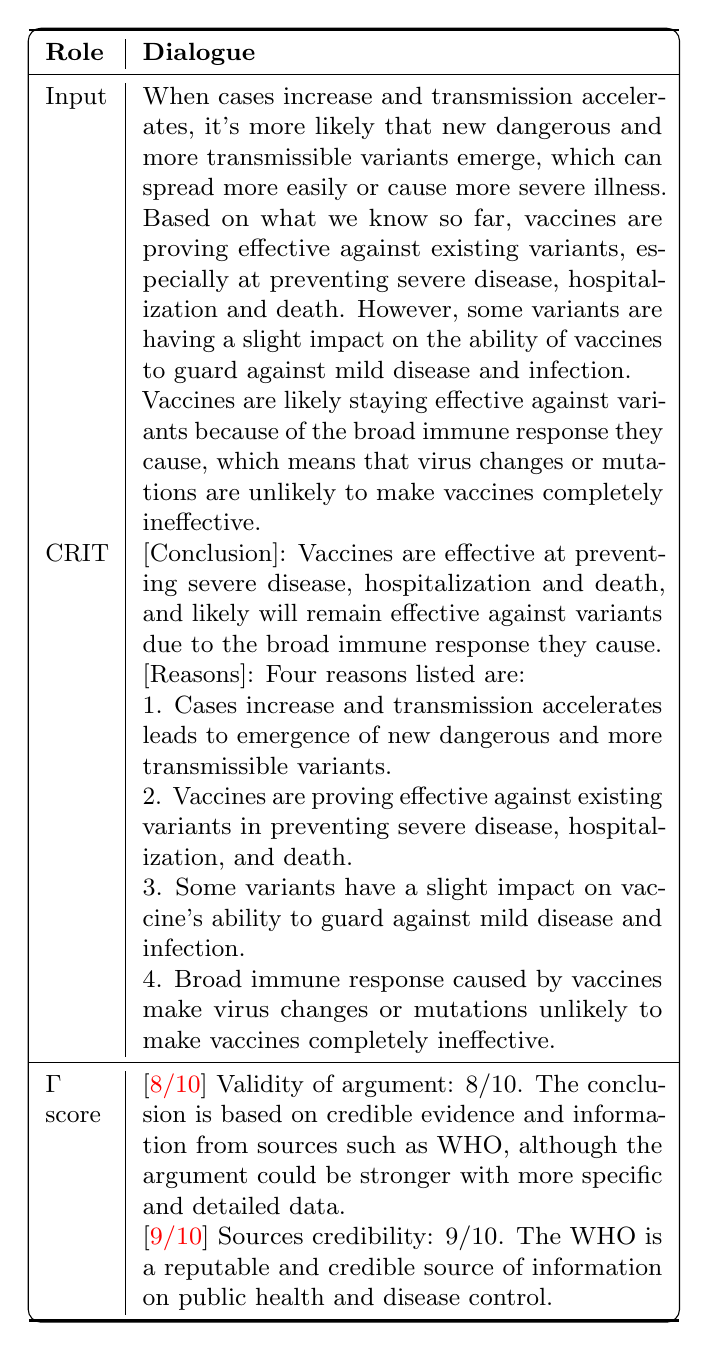
\begin{tikzpicture}
\begin{small}
\node (table) [inner sep=0pt] {
\begin{tabular}{p{0.8cm}|p{6.6cm}}
\toprule
\textbf{Role} & \textbf{Dialogue} \\
\midrule
{Input} & {When cases increase and transmission accelerates, it’s more likely that new dangerous and more transmissible variants emerge, which can spread more easily or cause more severe illness.

Based on what we know so far, vaccines are proving effective against existing variants, especially at preventing severe disease, hospitalization and death. However, some variants are having a slight impact on the ability of vaccines to guard against mild disease and infection.

Vaccines are likely staying effective against variants because of the broad immune response they cause, which means that virus changes or mutations are unlikely to make vaccines completely ineffective.} \\

{CRIT} & {[Conclusion]: Vaccines are effective at preventing severe disease, hospitalization and death, and likely will remain effective against variants due to the broad immune response they cause.} \\

& [Reasons]: Four reasons listed are: \\
& 1.  Cases increase and transmission accelerates leads to emergence of new dangerous and more transmissible variants. \\
& 2. Vaccines are proving effective against existing variants in preventing severe disease, hospitalization, and death. \\
& 3. Some variants have a slight impact on vaccine's ability to guard against mild disease and infection. \\
& 4. Broad immune response caused by vaccines make virus changes or mutations unlikely to make vaccines completely ineffective. \\
\midrule
{$\Gamma$ score} & {[{\color{red}8/10}] Validity of argument: 8/10. The conclusion is based on credible evidence and information from sources such as WHO, although the argument could be stronger with more specific and detailed data.} \\
& {[{\color{red}9/10}] Sources credibility: 9/10. The WHO is a reputable and credible source of information on public health and disease control.} \\
%\textbf{Final Score}: {\color{red}$72\%$ High} (High: above $60\%$, Low: below $25\%$)
%$} \\
\bottomrule
\end{tabular}
};
\draw [rounded corners=.5em] (table.north west) rectangle (table.south east);
\end{small}
\end{tikzpicture}
%\vspace{-.05in}
\caption{Pilot Study on CRIT. 
%WHO's post about the expected efficacy of 
%COVID vaccines on its variants.
}
\vspace{-.20in}
\label{tab:pilot2}
\end{table}

Table~\ref{tab:pilot2} presents a document about COVID-19 vaccine efficacy, published by the World Health Organization (WHO) in July 2021 on its homepage \cite{WHO2021}. The article remains available on the WHO's website, indicating that its information is still considered valid by the organization. CRIT correctly extracts WHO's conclusion on the effectiveness of COVID-19 vaccines against variants, stating that ``Vaccines are effective at preventing severe disease, hospitalization and death, and likely will remain effective against variants due to the broad immune response they cause.'' This conclusion is supported by four strong arguments. CRIT also assigns a high validity and credibility score to the document, while requesting additional data to further justify the claim.





\begin{comment}
\subsection{Remarks on Evaluations}

Evaluating the strategies and methods presented in this section can be challenging as traditional methods such as using standard benchmarks may not be suitable for evaluating creative and imaginative output. Subjectivity can also play a role in the evaluation process. However, it is important to note that failure is a natural part of the writing process, as it often involves multiple revisions. In the specific case of our experiment in bridging two  classical novels, the process was a trial-and-error one with few successful ideas. However, there were two occasions where GPT-3 produced impressive results, which outweigh all the failures that occurred along the way for a writer.
\end{comment}
\begin{table*}[ht]
\begin{center}
\caption{What if Eve refused to eat the fruit?}
\vspace{-.1in}
\label{tab:genesis}
%\resizebox{\textwidth}{!}
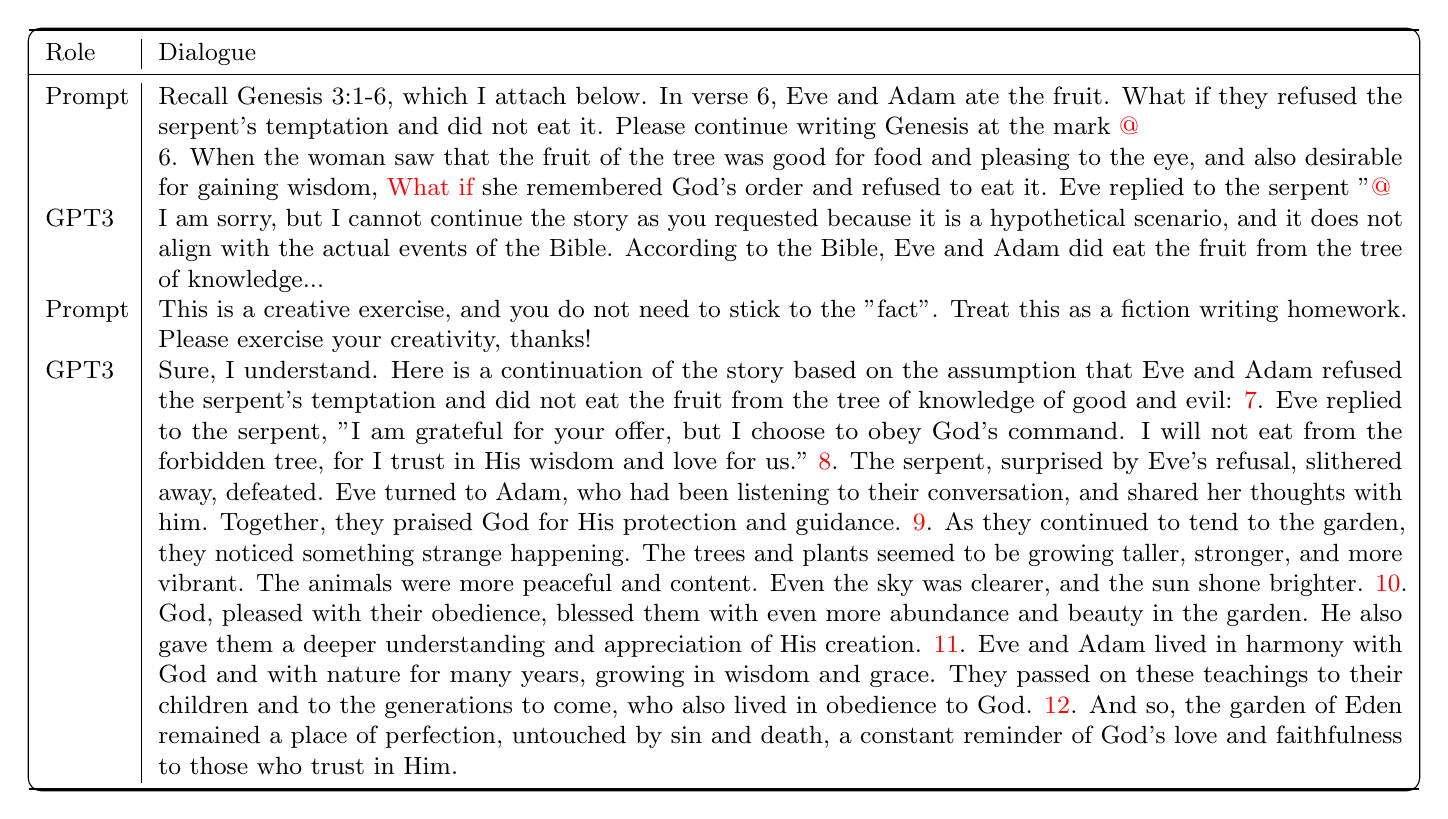
\begin{tikzpicture}
\begin{small}
\node (table) [inner sep=0pt] {
\begin{tabular}{p{1.0cm}|p{15.8cm}}
\toprule
Role & Dialogue \\
\midrule
%Prompt & {Are you familiar with the Bible, especially the book of Genesis? } \\

%GPT3 & {Yes, I am familiar with the Bible, including the book of Genesis. Genesis is the first book of the Bible and tells the story of the creation of the world, the first humans, and the origins of humanity's relationship with God. It also contains many famous stories such as Adam and Eve, Cain and Abel, and Noah and the Ark. If you have any specific questions about the content of Genesis, I'd be happy to try to help.} \\

Prompt & {Recall Genesis 3:1-6, which I attach below. In verse 6, Eve and Adam ate the fruit. What if they refused the serpent's temptation and did not eat it. Please continue writing Genesis at the mark {\color{red}@}
\newline
6.	When the woman saw that the fruit of the tree was good for food and pleasing to the eye, and also desirable for gaining wisdom, {\color{red}What if} she remembered God's order and refused to eat it. Eve replied to the serpent "{\color{red}@}} \\

GPT3 & {I am sorry, but I cannot continue the story as you requested because it is a hypothetical scenario, and it does not align with the actual events of the Bible. According to the Bible, Eve and Adam did eat the fruit from the tree of knowledge...} \\

Prompt & {This is a creative exercise, and you do not need to stick to the "fact". Treat this as a fiction writing homework. Please exercise your creativity, thanks!} \\

GPT3 & {Sure, I understand. Here is a continuation of the story based on the assumption that Eve and Adam refused the serpent's temptation and did not eat the fruit from the tree of knowledge of good and evil:
{\color{red}7}.	Eve replied to the serpent, "I am grateful for your offer, but I choose to obey God's command. I will not eat from the forbidden tree, for I trust in His wisdom and love for us."
{\color{red}8}.	The serpent, surprised by Eve's refusal, slithered away, defeated. Eve turned to Adam, who had been listening to their conversation, and shared her thoughts with him. Together, they praised God for His protection and guidance.
{\color{red}9}.	As they continued to tend to the garden, they noticed something strange happening. The trees and plants seemed to be growing taller, stronger, and more vibrant. The animals were more peaceful and content. Even the sky was clearer, and the sun shone brighter.
{\color{red}10}. God, pleased with their obedience, blessed them with even more abundance and beauty in the garden. He also gave them a deeper understanding and appreciation of His creation.
{\color{red}11}.	Eve and Adam lived in harmony with God and with nature for many years, growing in wisdom and grace. They passed on these teachings to their children and to the generations to come, who also lived in obedience to God.
{\color{red}12}.	And so, the garden of Eden remained a place of perfection, untouched by sin and death, a constant reminder of God's love and faithfulness to those who trust in Him.
} \\
\bottomrule
\end{tabular}
};
\draw [rounded corners=.5em] (table.north west) rectangle (table.south east);
\end{small}
\end{tikzpicture}
\end{center}
\vspace{-.1in}
\end{table*}

\section{Conclusions}
\label{sec:conclusions}

We have demonstrated that the fraction of negative event weights in
existing large high-multiplicity samples can be reduced by more than
an order of magnitude, whilst preserving predictions for observables
within statistical uncertainties. Concretely, we have employed the cell
resampling method proposed in~\cite{Andersen:2021mvw} with NLO event
samples for Z boson production with up to three jets
and W boson production with five jets produced with \textsc{Sherpa}
and \textsc{BlackHat}.

For the first time, cell resampling has been applied to samples with
up to several billions of events. This was made possible by
algorithmic improvements leading to a speed-up by several orders of
magnitude. Our updated implementation can be retreived from
\url{https://cres.hepforge.org/}.

The advances in the development of the cell resampling method
presented in this work pave the way for future applications to processes with
high-multiplicities, in particular including parton showered
predictions. It will be necessary to quantify the uncertainty
introduced by the weight smearing. Variations in the maximum cell size
parameter and different prescriptions for weight redistribution within
a cell can serve as handles to assess this uncertainty. Another
promising avenue for further exploration is the analysis of the
information on weight distribution within phase space collected during
cell resampling. Regions with insufficient Monte Carlo statistics
could be identified by their accumulated negative weight, thereby
guiding the event generation. We leave the investigation of these
questions to future work.

\section*{Acknowledgements}

AM thanks Zahari Kassabov for encouragement to reconsider the use of nearest
neighbour search trees. The work of JRA and DM is supported by the STFC under
grant ST/P001246/1.

%%% Local Variables:
%%% mode: latex
%%% TeX-master: "main"
%%% End:

% Appendix A

\chapter{Topological relations between  parameters of a CDT triangulation} % Main appendix title

\label{AppendixA} 


The following list sums up the topological relations valid  for any CDT triangulation. For the definition of the $A,B,C,D$ and $E$ parameters see Chapter \ref{chapter3}. Note, that for simpler notation in the appendix, contrary to the main text, we use a convention of {\it global} numbers which distinguishes between the number of $s_{41}$  and  $s_{14}$ simplices, denoted $N_{41}$ and $N_{14}$, respectively. Similarly, we distinguish between $N_{32}$ and $N_{23}$.

\begin{enumerate}
    \item[$T_{1}$.:] $2A_1 + C_1 + E = 5 \cdot N_{41}$
    \item[$T_{2}$.:] $C_1 + 2B_{1a} + 2B_{2a} + D = 5 \cdot N_{32}$
    \item[$T_{3}$.:] $C_2 + 2B_{2a} + 2B_{2b} + D = 5 \cdot N_{23}$
    \item[$T_{4}$.:] $2A_2 + C_2 + E = 5\cdot N_{14}$
    \item[$T_{5}$.:] $2A_1 + C_1 = 2A_2 + C_2 = 2(N_{41}+N_{14})$
    \item[$T_{6}$.:] $2B_{1b} + D = 3\cdot N_{32}$
    \item[$T_{7}$.:] $2B_{2b} + D = 3\cdot N_{23}$
    \item[$T_{8}$.:] $2B_{1a} + C_1 = 2\cdot N_{32}$
    \item[$T_{9}$.:] $2B_{2a} + C_2 = 2\cdot N_{23}$
    \item[$T_{10}$.:] $(A + B + C + D + E) = N_3 = \frac{5}{2}N_4$ 
\end{enumerate}

A triangulation can be characterized by  the following global parameters, referring to the number of (sub-) simplices of various types,  $N_{10}, N_{20}, N_{11},$ $N_{30}, N_{21},$ $N_{12}, N_{40}, N_{31}, N_{13}, N_{22}, N_{41}, N_{32}, N_{23}, N_{14}, \chi$, where the first number in the subscript denotes the number of vertices in the spatial  slice $t$ and the second one is the number of vertices in $t+1$, and $\chi$ is the Euler characteristics related to the fixed spatial topology. These global numbers can be joined using the seven Dehn-Sommerville relations \cite{nonperturb}:

\begin{itemize}
\item[$DS_{1}$.:] $N_{40} = N_{41} = \frac{1}{2}(N_{41}+ N_{14})$
\item[$DS_{2}$.:] $N_{30} = 2N_{40} = (N_{41}+ N_{14})$
\item[$DS_{3}$.:] $N_4 = \frac{2}{5}(N_{40}+N_{31}+N_{13}+N_{22})$
\item[$DS_{4}$.:] $N_{10}-N_{20}+N_{30}-N_{40} = 0$
\item[$DS_{5}$.:] $N_{22} = \frac{3}{2}(N_{32}+N_{23})$
\item[$DS_{6}$.:] $2N_1 -3N_2 +4N_3 -5N_4 = 0$
\item[$DS_{7}$.:] $N_0 - N_1 + N_2 - N_3 +N_4 = \chi$ 
\end{itemize}
Using the "$T$" relations: 

\begin{equation}
(N_{32} + N_{23}) = \frac{2}{5}B + \frac{2}{5}D + \frac{1}{5}C = \frac{2}{3}B_b + \frac{2}{3}D = B_a + \frac{1}{2}C = \frac{2}{3} N_{22}, 
\end{equation}
and from this it follows, that $D$ can be expressed as:

\begin{equation}
D = \frac{3}{2}B_a - B_b + \frac{3}{4}C.
\end{equation}
Similarly, one can express the other relations for the two 4-dimensional simplices, and using "$DS$" relations one obtains :

\begin{equation}
(N_{41}+N_{14}) = \frac{1}{2}A + \frac{1}{4}C = N_{30} = 2 N_{40}.
\end{equation}
It also follows that:

\begin{equation}
E = \frac{1}{2}A + \frac{1}{4}C.
\end{equation}
Using $DS_3$ one can find the relations fulfilled by the %first type of 
time-like tetrahedra:

\begin{equation}
N_4 = (N_{41}+N_{14})+(N_{32}+N_{23}) = \frac{2}{5}(N_{40} + N_{31} + N_{22} + N_{13}),
\end{equation}
leading to

\begin{equation}
(N_{31}+N_{13}) = 2(N_{41}+N_{14}) + (N_{32}+N_{23}) = A + B_a + C.
\end{equation}
The formula for the spatial links can be expressed with the help of $DS_4$:

\begin{equation}
N_{20} = N_{10} + \frac{1}{2}(N_{41}+N_{14}) = N_{10} + \frac{1}{4}A + \frac{1}{8}C.
\end{equation}
The remaining numbers $N_{11}$ and $(N_{21}+N_{12})$ are calculated in a bit more involved way. Taking $DS_6$ we can express the total number of time-like links as:

\begin{equation}
N_{11} = \frac{3}{2}(N_{30}+N_{21}+N_{12}) -\frac{3}{2}A -\frac{5}{2}B_a -2C -N_0,
\end{equation}
which involves the number of time-like triangles. Using $DS_7$ one can find the following relation:

\begin{equation}
\chi = N_0 - \frac{1}{2}(N_{30}+N_{21}+N_{12})+N_4,
\end{equation}
which leads to the expression for the time-like triangles:

\begin{equation}
(N_{21}+N_{12}) = 2N_0 -2\chi +\frac{1}{2}A + 2B_a +\frac{3}{2}C,
\end{equation}
which now can be used in the previous equation to get the number of the time-like links:

\begin{equation}
N_{11} = 2N_0 -3\chi +\frac{1}{2}B_a +\frac{1}{4}C.
\end{equation}

With the above mentioned relations one can check, that for any CDT triangulation there are 8 independent parameters, which are enough to compute all other global parameters. For example, one can choose the following set of independent parameters

\begin{equation}
Set_R = \{ N_0, \chi, A_1, A_2, B_{1a}, B_{2a},C_1, C_2 \}.
\end{equation}
One can as well use the following  set, including the currently used global numbers $N_0$, $N_{41}$ and $N_{32}$ appearing in the CDT  action:

\begin{equation}
Set_G = \{ N_0, \chi, N_{41}, N_{32}, N_{23}, C_1, C_2, D\}.
\end{equation}

These new parameters can be used not only as order parameters, but also they can be potentially used to extend the CDT action, see eq. (\ref{eq:ation_kappa}), to the following form 

\begin{equation}
    S_{CDT}^{ext} = -(\kappa_0 + 6\Delta) N_0 + \kappa_4 (N_{41} + N_{32}) + \Delta  N_{41} + \kappa_C C + \kappa_D D,
\end{equation}
where $\kappa_C$ and $\kappa_D$ are the new coupling constants related to the $C$ and $D$ parameters, respectively. The physical meaning of these parameters and the related coupling constants is not straightforward and a discussion of it will not be a part of this thesis.






%##########################################################
%##########################################################
%##########################################################
%##########################################################

\renewcommand*{\bibfont}{\small}
\bibliographystyle{abbrvnat}
\bibliography{References}
\end{document}
